%----------------------------------------------------------------------------------------
%	PACKAGES AND OTHER DOCUMENT CONFIGURATIONS
%----------------------------------------------------------------------------------------

\documentclass[11pt,fleqn]{book} % Default font size and left-justified equations
\setcounter{secnumdepth}{4}
\setcounter{tocdepth}{4}
\usepackage[top=3cm,bottom=3cm,left=3.2cm,right=3.2cm,headsep=10pt,a4paper]{geometry} % Page margins

\usepackage{xcolor} % Required for specifying colors by name
\definecolor{ocre}{RGB}{243,102,25} % Define the orange color used for highlighting throughout the book

% Font Settings
\usepackage{avant} % Use the Avantgarde font for headings
%\usepackage{times} % Use the Times font for headings
\usepackage{mathptmx} % Use the Adobe Times Roman as the default text font together with math symbols from the Sym­bol, Chancery and Com­puter Modern fonts

\usepackage{microtype} % Slightly tweak font spacing for aesthetics
\usepackage[utf8]{inputenc} % Required for including letters with accents
\usepackage[T1]{fontenc} % Use 8-bit encoding that has 256 glyphs

% Bibliography
\usepackage[style=alphabetic,sorting=nyt,sortcites=true,autopunct=true,babel=hyphen,hyperref=true,abbreviate=false,backref=true,backend=biber]{biblatex}
\addbibresource{bibliography.bib} % BibTeX bibliography file
\defbibheading{bibempty}{}

% Index
\usepackage{calc} % For simpler calculation - used for spacing the index letter headings correctly
\usepackage{makeidx} % Required to make an index
\makeindex % Tells LaTeX to create the files required for indexing
\usepackage{verbatim}
\usepackage{graphicx}
\usepackage{array}
\newcolumntype{L}[1]{>{\raggedright\let\newline\\\arraybackslash\hspace{0pt}}m{#1}}
\usepackage{tabularx}
%----------------------------------------------------------------------------------------

\begin{document}
	%----------------------------------------------------------------------------------------
	%	TITLE PAGE
	%----------------------------------------------------------------------------------------
	\let\cleardoublepage\clearpage
	\begingroup
	\thispagestyle{empty}
	%\AddToShipoutPicture*{\put(6,5){\includegraphics[scale=1]{portal-energy-background}}} % Image background
	
	\centering
	\vspace*{9cm}
	\par\normalfont\fontsize{35}{35}\sffamily\selectfont
	Title\par % Book title
	\vspace*{1cm}
	{\Huge Wael ARFAOUI}\par % Author name
	\endgroup
	
	%----------------------------------------------------------------------------------------
	%	Thanks
	%----------------------------------------------------------------------------------------
	\frontmatter
	
	\addcontentsline{toc}{chapter}{Remerciements}
	
	\begin{center}
		\vspace*{5cm}
		\par\normalfont\fontsize{20}{20}\sffamily\selectfont
		Remerciements
		\par\normalfont\fontsize{14}{14}\sffamily\selectfont
		\vspace*{1cm}
		C’est avec plaisir que Nous réservons cette page en signe de gratitude et de profonde reconnaissance à tous ceux qui nous ont aidé à réaliser ce projet.Nous tenons à remercier le jury pour l’honneur qu’il nous a fait pour avoir accepté de juger notre travail. Nous exprimons notre gratitude tout particulièrement à M.Sami Bessaies pour son encadrement, son aide, sa disponibilité, ses conseils fructueux et ses encouragements qu’il nous a prodigué tout au long de ce projet.	Finalement, et avec beaucoup de respect, nous ne pouvons laisser cette occasion sans saluer chaleureusement tous nos enseignants de l’ENIT ainsi que nos collègues pour leur soutien moral.\par
	\end{center}
	
	
	
	%----------------------------------------------------------------------------------------
	%	summary
	%----------------------------------------------------------------------------------------
	\newpage
	\addcontentsline{toc}{chapter}{Résumé}
	\begin{center}
		\vspace*{5cm}
		\normalfont
		{\LARGE Résumé}
		\vspace*{1cm}
	\end{center}
	
	Le présent rapport décrit les différents taches effectuées tout au long de notre expérience comme stagiaire chez Poulina Group Holding. Durant ce stage de trois mois, Nous avons travaillé sur l'application Bware, application développée par Smartdata technology.\\
	Cette application est un moyen de prévention contre les différents problèmes de santé. L'utilisateur peut surveiller tous les risques qui menacent sa santé. Que ce soit la Pollution, le Pollen, la Grippe, la Varicelle ou la Gastro-entérite, Bware" l'informe continuellement du niveau du risque.\\
	
	Le travail demandé consistait à améliorer l'application en rajoutant des fonctionnalités pour les utilisateurs publiques et d'autres pour le suivi et le contrôle de l'application.\\
	
	\textbf{Mots clés} : Santé, Prévention, épidémie, risque, pollution, REST API, Spring Fraework, Ionic framework.\\
	
	
	%----------------------------------------------------------------------------------------
	%	glossary
	%----------------------------------------------------------------------------------------

	\newpage
	\addcontentsline{toc}{chapter}{Glossaire}
	\vspace*{4cm}	
	{\LARGE Glossaire}
	
	\vspace*{1cm}
	\begin{flushleft}
		API Application Programming Interface\\
		CSS Cascading Style Sheet\\
		ENIT Ecole Nationale d’Ingénieurs de Tunis\\
		HTML Hypertext Markup Language\\
		HTTP HyperText Transfer Protocol\\
		JSON JavaScript Object Notation\\
		REST Representational State Transfer\\
		UML Unified Modeling Langage\\
		URI Uniform Resource Identifier\\
	\end{flushleft}

	%----------------------------------------------------------------------------------------
	%	table of contents
	%----------------------------------------------------------------------------------------
	\newpage
	\let\cleardoublepage\clearpage
	\addcontentsline{toc}{chapter}{Liste des figures}
	\renewcommand\listfigurename{Liste des figures}
	\listoffigures
	
	\newpage
	\let\cleardoublepage\clearpage
	\addcontentsline{toc}{chapter}{Liste des tableaux}
	\renewcommand\listtablename{Liste des tableaux} 
	\listoftables
		
	\newpage
	\let\cleardoublepage\clearpage
	\addcontentsline{toc}{chapter}{Table des Matières}
	\renewcommand\contentsname{Table des Matières}
	\tableofcontents
	
	

	
	%----------------------------------------------------------------------------------------
	%	chapters
	%----------------------------------------------------------------------------------------
	\mainmatter
	\addcontentsline{toc}{chapter}{Introduction}
\chapter*{Introduction}

\qquad Le monde entier vie dans un état d'évolution et de croissance rapide mais cette croissance vient à un coût cher. Des centaines voire des milliers de menaces contre la santé et l'environnement apparaissent chaque jour.\\

Selon l’Organisation mondiale de la santé (OMS), 3 millions de personnes meurent tous les ans à cause de la pollution de l’air. En 2015, près de 19 milliards d’euros ont été consacrés à des soins de santé lié à la qualité de l’air et 1,2 milliard de journées de travail ont été perdues. Outre les dégâts causés par la pollution de l'air, de nouvelles virus et épidémies apparaissent annuellement contre lesquels l'immunité humaine n'est pas encore développée, ce qui résulte enfin à l'apparition des maladies et des réactions allergiques parfois mortelles.\\

Pour lutter contre les risques présentés ci-dessus la plupart des personnes a recourt aux moyens classiques comme les masques, les gants et les cache-cols pour se protéger contre les différents agents contagieux.\\

L'inconvénient majeur de ces moyens est que les individus sont incapables de savoir au paravent le niveau de pollution ou même l'existence d'un éventuel risque à leur proximité. Et prenant en compte que la météo ne s'intéresse généralement qu'à l'état climatique, les personnes allergiques et fragiles n'ont aucun moyen pour s'informer sur l'état de l'air environnant.\\

La présence d'un 

	\chapter{Présentation générale du projet}
\section*{Introduction}
\qquad Nous consacrerons le présent chapitre à la présentation du contexte général de notre Projet, commençant par l’explication de cadre général de projet et son objectif, puis nous attaquerons la partie liée à l’étude de l’existant. Finalement une clarification sur la méthodologie de travail sera entamée.

\section{Cadre du projet}

\qquad Durant notre formation d'ingénieur nous sommes menés à effectuer un stage d'été d'au moins deux mois. Le présent stage a été élaboré à Poulina Group Holding et il consiste à améliorer l'application Bware développée par Smartdata technology.

\subsection{Entreprise d'accueil} 

\qquad Le stage a été effectué au sein de Aster Training filiale du groupe Poulina.

\subsubsection{Poulina Group Holding} 

\qquad Poulina est un groupe industriel et de services tunisien. Originellement spécialisé dans l’agriculture, le groupe s’est peu à peu diversifié pour devenir le premier groupe à capitaux privés du pays.\\

Le groupe s’est organisé au fil des années autour d’une dizaine de métiers regroupant les pôles d’activités de la holding : immobilier, travaux publics, bois et biens d’équipement, produits de grande consommation, emballage, transformation de l’acier, commerce et services, matériaux de construction et intégration avicole.

\subsubsection{Aster Training}

\qquad La société Aster training est une filiale du groupe Poulina et son capital social s’élève à 145000 DT. Créée en 1996, la société Aster training assure les activités suivantes :
\begin{itemize}
	\item Organise des séminaires de formation en gestion, technique et informatique.
	\item Ingénierie informatique.
	\item Étude, conception et développements des logiciels informatiques.
	\item Étude et mise en place des réseaux informatiques.
	\item Infogérance.
	\item Audit et conseil informatiques.
\end{itemize}

\subsection{Objectif du projet}

\qquad Le but du projet est d'apporter des améliorations à l'application Bware développée par l'entreprise française Smart Data Technology. Ces amélioration toucheront la partie destinées aux clients finales, la partie serveur ainsi que la partie destinée au suivi et contrôle de l'application.

\section{Études de l'existant}

\qquad De nos jours, nous témoignons une expansion du marché des applications mobiles. Parmi ces applications on note la présence d'une catégorie destinée à la santé humaine avec un pourcentage de 1\% du marché des applications et qui voit un accroissement d'à peu près 50\% chaque année. Gardant à l'esprit la nécessité cruciale de ces applications pour certains utilisateurs que ce soit pour des raisons de suivi de leur performance physique ou leur état sanitaire (tension, glycémie, température interne ...), nous déduirons en que la catégorie santé et fitness est un marché très important dans le domaine des applications mobiles. Notre intérêt est d'étudier les applications de prévention contre la pollution. Ainsi plusieurs solutions s'offrent aux utilisateurs des mobiles garantissant le suivi du niveau de la pollution à savoir Air Visual, Plume Air Report.

\subsection{Analyse de l'existant}

\qquad Les solutions présentées ci-dessus ne couvrent pas l'intégralité des fonctionnalités nécessaires pour les utilisateurs mais elles en offrent d'autres telles que le partage de l'état de l'air dans les réseaux sociaux et la couverture des villes de partout dans le monde. Parmi les fonctionnalités absentes, nous citons :
\begin{itemize}
	\item Les notifications pour Air Visual
	\item Les détails sur les différents type de pollution pour Plume Air Report
	\item La présence de la carte
\end{itemize} 

\subsection{Critique de l'existant}

\qquad Les exemples cités précédemment ne permettent d'intégrer qu'une partie des fonctionnalités nécessaires pour le suivi du niveaux de la pollution dans des zones éparpillées dans le monde en raison d'une quarantaine de villes par pays. Nous citons aussi d'autres fonctionnalités absentes chez les concurrents telles que les notifications, les conseils et les détails sur les différents type de pollution.

\subsection{Solution proposée}

\qquad Notre solution consiste à couvrir les déficiences des applications présentées en mettant en place une application mobile multiplate-forme destinée aux utilisateurs français qui couvrira la totalité du territoire français mais qui permettra aussi de prévenir les utilisateurs des différents risques auxquels ils sont inscrits, d'afficher des détails sur les agents nocifs et des conseils concernant les niveaux de risque élevés.\\

\section{Méthodologie de travail}

\qquad Pour mener à bien notre projet nous avons opté pour une méthodologie afin d'organiser les différentes phases du projet.\\

Alors nous avons adopté l'approche agile qui consiste à un paradigme révolutionnaire dans le monde de gestion de projet. Cet approche diffère des méthodes classiques par la migration du centre d'intérêt des étapes par lesquels passe le projet vers les étapes par lesquels passe le produit. Ainsi, cet approche élimine l'effet tunnel pour donner davantage de visibilité et de transparence en impliquant le client dans  tous les procès de la réalisation. Ce qui résulte en des majeurs changements sur tout le processus de réalisation qui devient à la fois itératif et incrémental ce qui permettra une meilleure flexibilité aux niveaux de la spécification des besoins mais en gardant un minimum de règles.\\

\subsection{Méthode Scrum}

Au sein de ce cadre méthodologique de gestion de projet, les acteurs ajustent empiriquement, au fil des itérations, leur propre méthode en fonction de leur contexte. On peut qualifier Scrum de simple, pragmatique, transparent et empirique. Scrum ne couvrant que les aspects de gestion de projet, c’est souvent la méthodeeXtreme Programming (XP) qui vient compléter le vide laissé en matière de pratiques de développement. XP apporte ainsi les pratiques de programmation en binôme, de développement piloté par les tests (TDD ou Test Driven Development), intégration continue, etc.\\
Le cycle préconisé par TDD comporte cinq étapes.
   \begin{itemize}
   	\item Écrire un premier test ;
   	\item Vérifier qu’il échoue (car le code qu’il teste n’existe pas), afin de vérifier que le test est valide ;
   	\item Écrire juste le code suffisant pour passer le test ;
   	\item Vérifier que le test passe ;
   	\item Puis ré-usiner le code, c’est-à-dire l’améliorer tout en gardant les mêmes fonctionnalités
   \end{itemize}

\section*{Conclusion}

\qquad Dans ce chapitre, nous avons présenté le cadre général de notre stage en énonçant notre entreprise d’accueil et les objectifs envisagés de ce stage. Nous nous sommes intéressés, par la suite, à l’analyse et la critique des solutions similaires déjà existantes dans le marché et à la proposition de notre solution alternative.

	\chapter{Analyse et spécification des besoins}

\section*{Introduction}

\qquad Après avoir présenté le contexte général de notre projet, nous venons d’énoncer dans cette partie les besoins auxquels notre application devra réponde. Nous énumérerons les besoins fonctionnels et non fonctionnels dans une première partie et nous exposerons par la suite la spécification de ces besoins à travers les diagrammes de cas d’utilisation.

\section{Analyse des besoins}

\qquad Ce chapitre est dédié à l'étude profonde des différents besoins sur l'échelle fonctionnelle et non fonctionnelle. Nous projetons de détailler les risques et contraintes auxquelles est soumis notre projet dans le but de répondre aux besoins.

\subsection{Identification des acteurs}

\qquad L'application doit garantir la prévention contre les risques de pollution pour l'utilisateur final et la suivi et contrôle pour les administrateurs de Smartdata.

\subsection{Besoins fonctionnels}
\qquad Nous présentons ci-dessous les besoins fonctionnels regroupés par acteur:

\begin{itemize}
	\item Utilisateur
		\begin{itemize}
			\item Visualisation des niveaux des risques
			\item Inscription aux différents risques
			\item Visualisation des détails sur les risques
			\item Visualisation des états des stations
			\item Visualisation des conseils
			\item Inscription aux rappels santé
			\item Ajout d'astuces
		\end{itemize}
	\item Administrateur
		\begin{itemize}
			\item Consultation des statistiques
			\item Réception des Emails concernant les batchs
			\item Réception des Emails concernant les notifications
		\end{itemize}
\end{itemize}

\subsection{Besoins non fonctionnels}

\qquad Pour bien répondre à ses besoins notre application doit respecter les exigences techniques suivantes: 

\textbf{Ergonomie} Le but de l’application est qu’elle soit exploitée par des simples utilisateurs qui ne sont pas forcément expérimentés dans le domaine de l’informatique, et qu’elle le soit de la façon la plus efficace. Les interfaces de l’application doivent être ergonomiques et conviviales.

\textbf{Environnement et architecture} L’application doit être mise en place dans une architecture répartie multi-tiers et accessible via le Web à travers les navigateurs Web.

\textbf{Rapidité} Notre application doit garantir un accès rapide aux données et d’une manière transparente.

\textbf{Scalabilité} L’application doit être facilement extensible pour pouvoir accueillir un public plus large.

\textbf{Documentation} L’application sera livrée avec une documentation des différentes fonctions et API qu’elle offre, nécessaire pour les futurs développeur

\section{Spécification des besoins}

\qquad Dans ce paragraphe, nous allons préciser les différents besoins de notre application en ayant recours au langage de modélisations UML. Nous illustrons les besoins par les diagrammes de cas d'utilisation.

\subsection{Diagramme de cas d'utilisation global}

\qquad Nous présentons dans cette partie le diagramme de cas d'utilisation global de notre application. La figure \ref{fig2.1} représente le diagramme de cas d'utilisation global.

\begin{figure}[!h]

	\begin{center}
		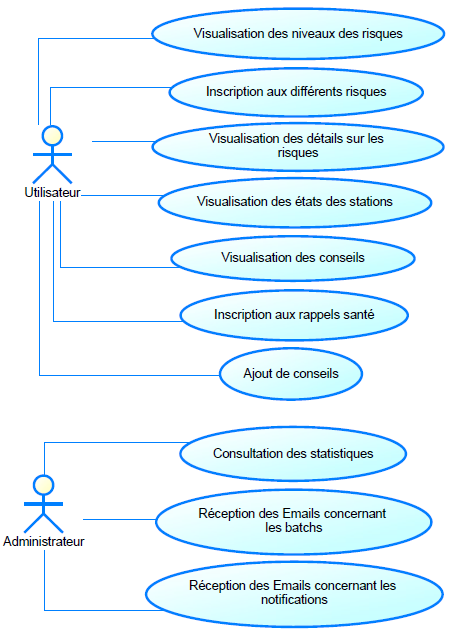
\includegraphics[width =7.1cm ]{figures/globalusecase}		
	\end{center}
	\caption{Diagramme des cas d'utilisation global}
	\label{fig2.1}
\end{figure}

\subsection{Raffinement des cas d'utilisation}

\qquad Dans cette partie, nous présentons les diagrammes de cas d'utilisation raffinés. Nous détaillerons quelques cas d'utilisation parmi ceux qui sont précédemment présentés. 

\subsubsection{Cas d'utilisation : Ajouter astuces}

\qquad La figure \ref{fig2.2} représente le diagramme de cas d'utilisation de l'ajout des astuces.

\begin{figure}[!h]
	\begin{center}
		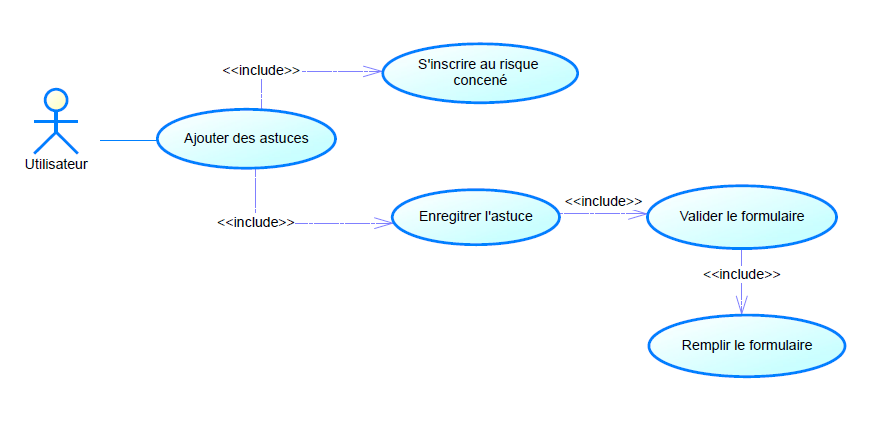
\includegraphics[width=0.64\textheight]{figures/uc_ajoutastuce}
	\end{center}
	\caption{Cas d'utilisation : Ajouter des astuces}
	\label{fig2.2}
\end{figure}

Ci-dessous une description sous forme de tableau du cas d'utilisation : Ajouter astuce.

\begin{table}[!h]
	\caption{Description textuelle du cas d'utilisation : Ajouter astuce}
	\begin{center}
		\begin{tabular}{|L{4cm}|L{10cm}|}
			\hline
			\textbf{Cas d’utilisation} & Ajouter astuce\\
			\hline
			\textbf{Objectif} & Permettre d'ajouter des astuces\\
			\hline
			\textbf{Acteur} & Utilisateur\\
			\hline
			\textbf{Pré-conditions} & S'inscrire, remplir et valider le formulaire\\
			\hline
			\textbf{Post-condition} & Astuce ajoutée\\
			\hline			
			\textbf{Scénarios nominaux} & \textbf{S1. Soumettre une astuce} L'utilisateur remplie le formulaire d'ajout d'astuces, choisit le type de risque, saisit son adresse électronique enfin il confirme l'ajout par cliquer sur le bouton enregistrer\\
			\hline
			\textbf{Exceptions} & \textbf{E1} Utilisateur non inscrit au risque.\\ &\textbf{E2} L'un des champs du formulaire est soit vide soit non valide.\\
			\hline
		\end{tabular}
	\end{center}
\end{table}

\section*{Conclusion}

\qquad Nous avons consacré ce chapitre, à la spécification des besoins, ce qui permet de mieux comprendre les problématiques soulevées et d’avoir une vue globale sur les fonctionnalités constituantes notre projet. Nous nous intéressons dans le chapitre suivant aux éléments de conception basée sur le travail effectué dans le présent chapitre.
\end{document}